\section{Resultados}
\begin{frame}
\frametitle{Anti-thickness geométrico}
Para $3 \leq n \leq 10$:
\[  At_g(K_n) = n - \left\lfloor\sqrt{2n + \frac{1}{4}} - \frac{1}{2} \right\rfloor \]
\end{frame}
\begin{frame}
\frametitle{Estado del arte}
Para $n \geq 3$:
\[  \frac{n-1}{2} \leq At_g(K_n) \leq n - \left\lfloor\sqrt{2n + \frac{1}{4}} - \frac{1}{2} \right\rfloor \]
Para encontrar alguna cota inferior es posible explotar alguna propiedad que se cumpla para todas las gráficas geométricas de $K_n$. Para encontrar una cota superior es posible ofrecer una descomposición de $K_n$ en thrackles.
\end{frame}
\begin{frame}
\frametitle{Estado del arte : cota inferior}
Erd\H{o}s \emph{et al.}(1988) probaron que cada gráfica geométrica con $n$ vértices en la cual no existen dos aristas disjuntas tiene a lo sumo $n$ aristas. 
\\[10pt]
Esto quiere decir que un thrackle máximo tiene a lo sumo $n$ aristas.
\end{frame}
\begin{frame}
\frametitle{Estado del arte : cota inferior}
En el trabajo de Wood \& Dujmovic se menciona que para $n \geq 3$:
\[  \frac{n-1}{2} \leq At_g(K_n).\] 
\pause

Esta cota inferior es la más sencilla, se basa en la noción del número máximo de aristas en un thrackle máximo. 
\\[5pt]
Si la gráfica completa tiene $\binom{n}{2} = \frac{n(n-1)}{2}$ aristas, ¿cuántos thrackles máximos son necesarios para \emph{cubrir} todas las aristas? Si suponemos que $k$ thrackles máximos\footnote{En el mejor caso, una descomposición por thrackles es inducida por una colección de thrackles máximos.} son necesarios la siguiente desigualdad nos otorga el resultado si resolvemos para $k$: \[ k\cdot n \geq \frac{n(n-1)}{2} \pause \Rightarrow k = \frac{n-1}{2}\]
\end{frame}

\begin{frame}
\frametitle{Estado del arte : cota superior}
Fabila-Monroy \emph{et al.} encuentran el anti-thickness exacto cuando $S$ está en posición convexa. Ellos estudian el problema del anti-thickness desde número cromático de $D(S)$. Para la cota inferior establecen el número mínimo de colores necesarios en una coloración propia de $D(S)$ y para la cota superior dan una coloración propia para cualquier $n$, con $n>3$.
\pause 
\\[10pt]
Ellos establecen que $\chi(D(S)) = n - \left\lfloor\sqrt{2n + \frac{1}{4}} - \frac{1}{2} \right\rfloor, $ cuando $S$ está en posición convexa.
\pause
\\[10pt]
Como la posición convexa es un dibujo de $K_n$ tenemos: \[At_g(K_n) \leq n - \left\lfloor\sqrt{2n + \frac{1}{4}} - \frac{1}{2} \right\rfloor. \]
\end{frame}
\begin{frame}
\frametitle{Estado del arte : thrackles máximos en posición convexa}
Un resultado del trabajo de Fabila-Monroy \emph{et al.} es que prueban que dos thrackles máximos en posición convexa siempre comparten al menos una arista. Esto significa que, en posición convexa y en el mejor caso, una colección de $k$ thrackles máximos cubre a lo sumo $kn - \binom{k}{2}$ aristas. Para obtener el valor más pequeño de $k$ podemos resolver, para $k$, la siguiente desigualdad :
\[
  kn - \binom{k}{2} \geq \binom{n}{2}.
\]
Usando la ecuación cuadrática encontramos que $k = n - \left\lfloor\sqrt{2n + \frac{1}{4}} - \frac{1}{2} \right\rfloor.$
\end{frame}
\begin{frame}
\begin{figure}
	\centering
	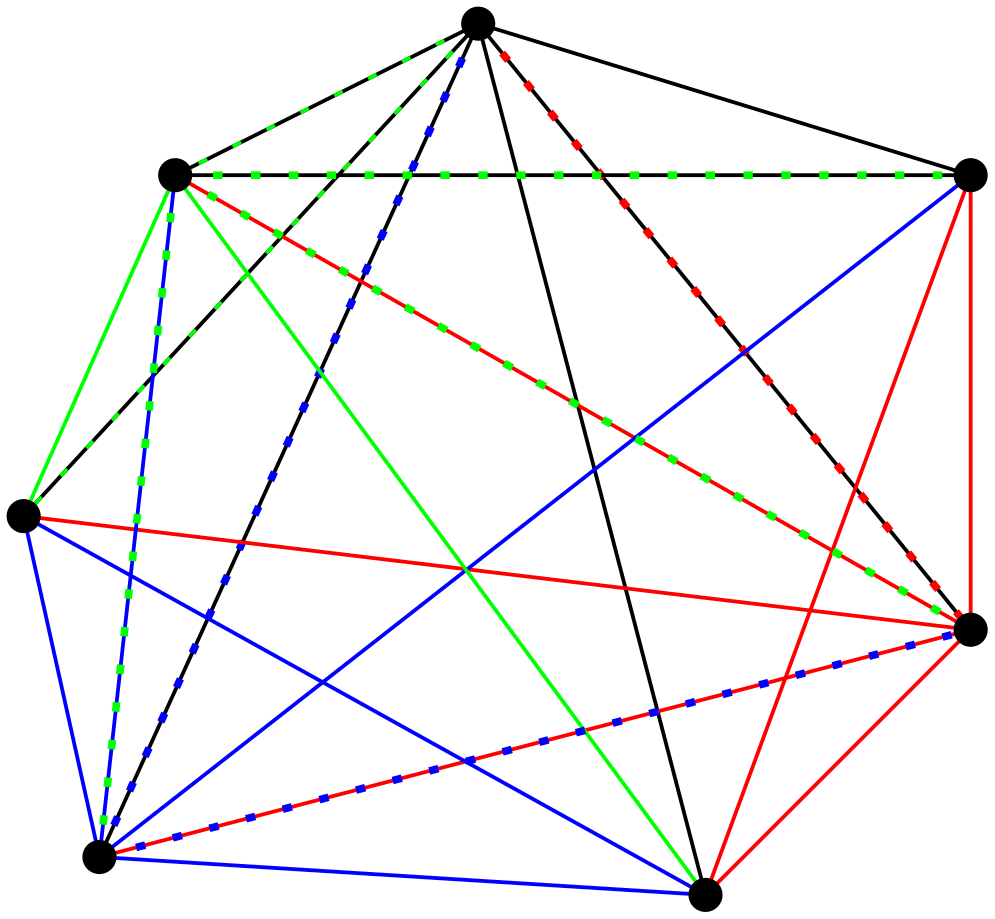
\includegraphics[width=0.75\linewidth]{images/thrackles_maximos}
\end{figure}
\end{frame}

\begin{frame}
\frametitle{Estado del arte : thrackles máximos en posición general}
\pause
\begin{itemize}
	\item En posición general es muy dificil dibujar thrackles máximos que sean disjuntos.
	\item La intuición nos dice que el resultado anterior es válido para posición general.
	\item ¿Cómo probamos \emph{todas} las gráficas geométricas de $K_n$?
\end{itemize}
\end{frame}

\begin{frame}
\frametitle{Tipo de orden}
Aichholzer \emph{et al.} definen el \emph{tipo de orden} de un conjunto $S=\{p_1,p_2,\dots p_n\}$ de puntos en posición general
como una función que asigna a cada tripleta ordenada $i,j,k\in\{1,2,\dots n\}$ la orientación de la tripleta de puntos $\{p_i,p_j,p_k\}$.
\begin{figure}
	\centering
	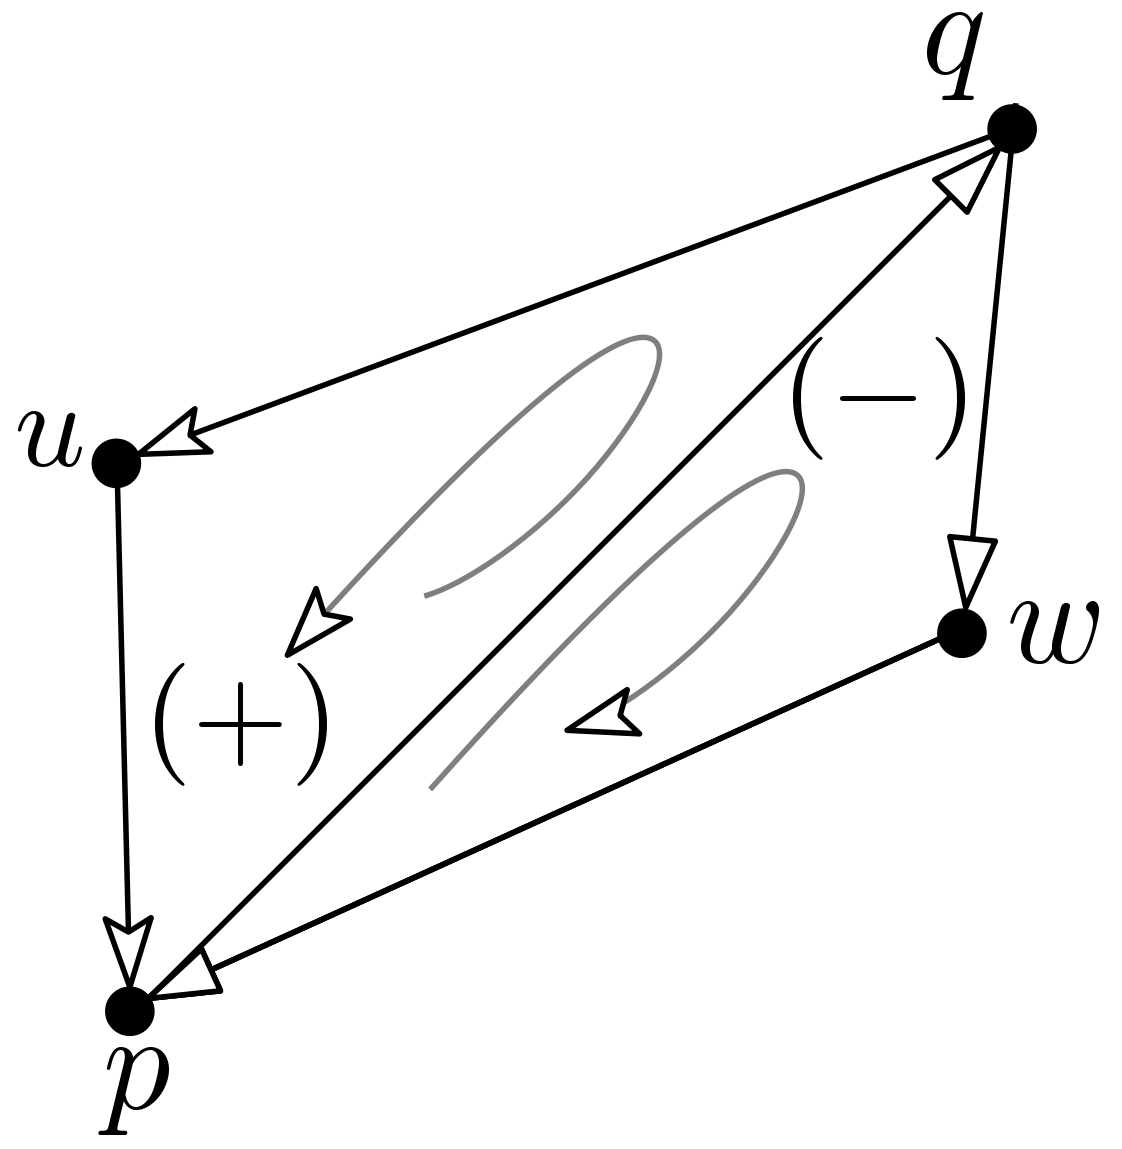
\includegraphics[width=0.3\linewidth]{images/triplet}
\end{figure}
Decimos que dos conjuntos de puntos $S_1$ y $S_2$ son combinatoriamente equivalentes cuando tienen el mismo tipo de orden.
\end{frame}

\begin{frame}
\frametitle{Tipo de orden}
Aichholzer \emph{et al.} ofrecen una base de datos para los tipos de orden de $3 \leq n \leq 10$.
\begin{table}[ht]
	\centering
	\begin{tabular}{|c|c|r|}
		\hline
		$n$ & Número de tipos de orden & Tamaño (bytes)   \\ \hline
		3     & 1                   & 6       \\ \hline
		4     & 2                   & 16      \\ \hline
		5     & 3                   & 30      \\ \hline
		6     & 16                  & 192     \\ \hline
		7     & 135                 & 1890    \\ \hline
		8     & 3315                & 53040   \\ \hline
		9     & 158817              & 5 717 412   \\\hline
		10    & 14309547            & 572 381 880 \\ \hline
	\end{tabular}
	\caption{Tipos de orden para cada $n\leq10$.}
	\label{tab:ots}
\end{table}
\end{frame}
\begin{frame}
\frametitle{Estado del arte : construyendo la nueva cota inferior}
Para analizar cada par de thrackles máximos en algun dibujo de $K_n$, primero hay que encontrarlos. Por ello, construimos un algoritmo 
exhaustivo que usa \emph{backtracking} para encontrar thrackles de cualquier tamaño. Nosotros llamamos $k-$thrackle a un thrackle de tamaño $k$.
Explicar algoritmo de búsqueda de $k$ thrackles y cómo hacemos la intersección.

\end{frame}

\begin{frame}
\frametitle{Estado del arte : construyendo la nueva cota inferior}
Una vez que hicimos las intersecciones de cada par de thrackles máximos en todos los dibujos de $K_n$, con $3 \leq n \leq 10$ encontramos los siguientes resultados:
\begin{itemize}
	\item Para todo tipo de orden con al menos dos thrackles máximos, cada par de thrackles máximos tienen intersección no vacía en aristas.
	\item Existen tipos de orden con solo un thrackle máximo.
	\item Existen tipos de orden en los que no hay thrackles máximos.
\end{itemize}
\end{frame}

\begin{frame}
\frametitle{Estado del arte : construyendo la nueva cota inferior}
Esto nos permite calcular el número exacto de aristas cubiertas, en el mejor caso, por una descomposición que es inducida por una colección de thrackles máximos. 

Nosotros probamos que, $m$ thrackles máximos pueden cubrir a lo sumo:
\[
-\frac{1}{2}m(m-2n-1)
\] aristas de la gráfica completa.
\pause 

\begin{table}
	\centering
\scalebox{0.7}{

	\begin{tabular}{	| >{\centering\arraybackslash}m{0.5in} | >{\centering\arraybackslash}m{0.8in} |  >{\centering\arraybackslash}m{1.2in} |  >{\centering\arraybackslash}m{1in} | }
		\hline
		$n$ & $m = \left\lceil\frac{n-1}{2}\right\rceil$ &     $-\frac{1}{2}m(m-2n-1) $ &
		$\binom{n}{2}$\\[5pt] \hline\hline
		3   & 1  & 3 & 3 \\ \hline
		4   & 2  & 7 & 6 \\ \hline
		5   & 2  & \cellcolor{red!25}9 & 10 \\ \hline
		6   & 3  & 15 & 15 \\ \hline
		7   & 3  & \cellcolor{red!25}18 & 21 \\ \hline
		8   & 4  & \cellcolor{red!25}26 & 28 \\ \hline
		9   & 4  & \cellcolor{red!25}30 & 36 \\ \hline
		10  & 5  & \cellcolor{red!25}40 & 45 \\ \hline
	\end{tabular}
}
\end{table}
\end{frame}

\begin{frame}
\frametitle{Estado del arte : construyendo la nueva cota inferior}
De la misma manera, para saber cuántos thrackles son necesarios para cubrir todas las aristas de la gráfica completa, debemos 
resolver la siguiente desigualdad para $m$:
\[
-\frac{1}{2}m(m-2n-1) \geq \binom{n}{2}.
\]
Usando la ecuación cuadrática encontramos que \[m =  n - \left\lfloor\sqrt{2n + \frac{1}{4}} - \frac{1}{2} \right\rfloor \]

\end{frame}
\begin{frame}
\frametitle{Estado del arte : construyendo la nueva cota inferior}
\begin{table}
	\centering
	\scalebox{0.9}{
		
		\begin{tabular}{	| >{\centering\arraybackslash}m{0.5in} | >{\centering\arraybackslash}m{1.6in} |  >{\centering\arraybackslash}m{1.2in} |  >{\centering\arraybackslash}m{1in} | }
			\hline
			$n$ & $m =  n - \left\lfloor\sqrt{2n + \frac{1}{4}} - \frac{1}{2} \right\rfloor $ &     $-\frac{1}{2}m(m-2n-1) $ &
			$\binom{n}{2}$\\[5pt] \hline\hline
			3   & 1  & 3 & 3 \\ \hline
			4   & 2  & 7 & 6 \\ \hline
			5   & 3  & 12 & 10 \\ \hline
			6   & 3  & 15 & 15 \\ \hline
			7   & 4  & 22 & 21 \\ \hline
			8   & 5  & 30 & 28 \\ \hline
			9   & 6  & 39 & 36 \\ \hline
			10  & 6  & 45 & 45 \\ \hline
		\end{tabular}
	}
\end{table}
Tenemos una nueva cota inferior para $3 \leq n \leq 10$:
\[ At_g(K_n) \geq n - \left\lfloor\sqrt{2n + \frac{1}{4}} - \frac{1}{2} \right\rfloor \] 
\end{frame}
\begin{frame}
\frametitle{Anti-thickness geométrico de $K_n$ para $3\leq n\leq 10$}
Con el resultado anterior y el resultado del estado del arte tenemos que, para $ 3 \leq n \leq 10$:
\[ n - \left\lfloor\sqrt{2n + \frac{1}{4}} - \frac{1}{2} \right\rfloor  \leq At_g(K_n) \leq n - \left\lfloor\sqrt{2n + \frac{1}{4}} - \frac{1}{2} \right\rfloor \] 
\pause
\[ At_g(K_n) = n - \left\lfloor\sqrt{2n + \frac{1}{4}} - \frac{1}{2} \right\rfloor \] 
\end{frame}

\begin{frame}
\frametitle{Anti-thickness geométrico de $K_n$ para $3\leq n\leq 10$}
\begin{itemize}
	\item[] Recordemos que la cota superior fue obtenida encontrando el anti-thickness de un dibujo específico, el que está en posición convexa.
	\item[] Recordemos que si $S$ es un conjunto de $n$ vértices en posición convexa, entonces \[ At_g(K(S)) = \min\{D(S)\} = \max\{D(S)\} = d(n)\]
\end{itemize}
¿Qué pasa con el anti-thickness de dibujos en posición general no convexa?
\end{frame}

\begin{frame}
\frametitle{Anti-thickness de dibujos en posición general no convexa}
\end{frame}